\documentclass[11pt]{article}
\usepackage[toc,page]{appendix}
\usepackage{cite}
\usepackage{graphicx}
\usepackage{hyperref}
\usepackage{amsfonts}
\usepackage{listings}

\begin{document}

\title{Odefying Kirkham}
\author{Simon Johanning}
\date{\today}
\maketitle

\tableofcontents

\section{Introduction} \label{sec:Intro}
\subsection{Background}
This course work has been written in the context of the course "Modellierung biologischer und molekularer Systeme" (WS 2015/16) at the University of Leipzig.

It is based on a presentation of the paper \textit{Early gene regulation of osteogenesis in embronic stem cells} by \textit{G.R. Kirkham et. al.} (see \cite{Kirkham}) in the context of aforementioned course.

It will lay out the basic ideas of the paper (\ref{ssec:Kirkham}), give an overview of the mathematical ideas the methodology is based upon (\ref{sec:Theory}), and will discuss results from the investigation of the boolean networks, as well as their continuous homologues (\ref{sec:Results}). It will close with a discussion of the paper and the derived results (\ref{sec:Discussion}).

Since the course associated with this course work is about (mathematical) modeling, and the mathematical techniques used in the paper were merely sketched, this report will focus mostly on the mathematical ideas and modeling aspects employed in the paper, as well as the challenges in reproducing the results, and will only treat the biological context of \cite{Kirkham} on the side.
\subsection{Kirkham paper} \label{ssec:Kirkham}
\subsubsection{Motivation} \label{sssec:Motivationkirkham}
Motivated by the knowledge gap of networks regulating the differentiation of mouse embryonic stem cells into bone cells, the authors of \cite{Kirkham} are interested in understanding the regulatory mechanisms of osteogenesis.
Since mathematical models of gene regulatory networks (GRNs) have proven to characterize GRNs well, as well as making novel predictions, especially in the case of incomplete data, the authors investigate mathematical models suited for this application.

Since boolean models (BMs) capture the qualitative dynamics of biological systems in a number of studies, the authors chose to start out modeling the GRN under investigation with boolean models.
In order to capture the quantitative dynamics of the system under investigation, they then transform these BMs into their continuous homologue functions in order to describe the system as a set of ordinary differential equations (ODE), a process call "odefication", using the \href{http://www.helmholtz-muenchen.de/icb/software/odefy/index.html}{Odefy} toolbox.

This process is chosen since the description of a system through ODEs captures the dynamics of a system very well and helps the authors to identify a (unique) GRN, characterizing the influence of the transcription and growth factors under consideration.

\subsubsection{Structure}
As noted above, \cite{Kirkham} investigates GRNs relevant to osteogenesis in embryonic stem (ES) cells. Based on existing research on osteogenetic differentiation of mouse ES cells, they derive a set of three genes and two growth factors (GFs) to be of particular interest for this GRN, and aim to identify the relationship between them. 
These are the genes Runx2, Dlx5, Msx2 and the GFs TGF$\beta$1 and BMP2.

Consequently the authors test different GRNs involving these genes and GFs, narrowing down the possible candidates. 

Starting from modeling the GRNs as Boolean Models, they transform these into differential equations ("odefication") fitted to measured data in order to test predictions about the GRNs behaviour under over- and underexpression of the GFs. 

Their experimental data comprises a set of measurements of the TFs of interest (Dlx5, Msx2, Runx2) at 5 fixed time points, exposed to the GFs BMP2, TGF$\beta$1 and a combination of these.
The expression levels of the TFs were used to reduce the number of candidate GRNs through comparing the expression profiles to the stable states of the GRNs.

The remaining GRNs (i.e. the ones matching the experimental expression profiles) were then transformed into continuous ODEs, and their over- and underexpression behaviour was compared to experimental results, ruling out all but one network.

The paper closes with a discussion and the description of the experimental setup.

\section{Theory} \label{sec:Theory}
As mentioned in the \hyperref[sec:Intro]{Introduction}, \cite{Kirkham} starts out with boolean models\footnote{For an elaboration on BM see \ref{AppendixA}} of the species in the GRN. 

Boolean models (BMs) express qualitative biological knowledge and have shown quite fruitful for this purpose. Since however many approaches depend on a quantitative characterization of a system, the process of deriving quantitative behaviour from a qualitative description is of utmost importance.

As mentioned in the introduction, \cite{Kirkham} uses the process of 'odefication' in order to achieve a quantitative characterization of a system from a qualitative description (BM). Since \cite{Kirkham} is very brief about the mathematical aspects of this process, this course work will in the following lay out the mathematical ideas for this approach (as described in \cite{Wittmann} and \cite{Krumsiek}).

\subsection{General approach to make discrete models continuous} \label{ssec:prop}
In order to derive continuous models from the BMs $B_{i}$, continuous homologues of these have to be found. For this, the discrete variables $x_{i}$ are replaced by continous variables $\overline{x_{i}} \in [0, 1]$ , yielding the \textit{continuous homologue} functions $\overline{B_{i}} : [0, 1]^{N_{i}} \rightarrow [0, 1]$ on the unit interval.

Using the continous homologues of the BMs, the behavior of the species can be described through the differential equation

 $\dot{\overline{x_{i}}} = \frac{1}{\tau_{i}} (\overline{B}_{i} (\overline{x}_{i_{1}}, \overline{x}_{i_{2}},..., \overline{x}_{i_{N_{i}}}) - \overline{x}_{i})$,
 
 where the production of $\overline{x}_{i}$ is given by $\overline{B}_{i}$, and $\tau_{i} := \frac{1}{\gamma_{i}}$ stands for the life-time of species $X_{i}$, with $\gamma_{i}$ as the decay rate of $X_{i}$.

For the (in respect to the BM) homologuous continuous functions $\overline{B}_{i}$, three properties need to hold (as noted in \cite{Wittmann}):
\begin{itemize}
	\item \textbf{Accuracy}: $\overline{B_{i}}$ and $B_{i}$ need to agree on the vertices of the unit cube ($\{0,1\}^{N_{i}})$ \footnote{$\overline{B_{i}}$ are then called \textit{perfect} continuous homologues, exhibiting similar steady-state behavior}
	\item \textbf{Good analytical properties} such as smoothness, so a mathematical analysis as a system of ODEs can be performed
	\item \textbf{Minimality and uniqueness}: $\overline{B}_{i}$ should be the unique minimal solutions in their interpolation class
\end{itemize}

\subsubsection{HillCube} \label{sssec:Hillcube}
In order to achieve the desired properties sketched above, normalized \textit{HillCubes} are constructed. HillCubes employ \textit{Hill functions} on the edges of the unit cube described above for the functional behavior of the interpolations.
As a first step to arrive at (normalized) HillCubes, \textit{BooleCubes} are constructed. These are functions that interpolate $B_{i}$ linearly through the use of multivariate polynomial interpolation. In order to get a unique solution,
the function with the minimal degree (of the polynomial) is chosen. This function satisfies the properties set out in \ref{ssec:prop}.

The functions $\overline{B}_{i}^{I} (\overline{x}_{i_{1}}, \overline{x}_{i_{2}},..., \overline{x}_{i_{N_{i}}} )$ define a system of ODEs that describe the temporal development of $\overline{x}_{i}$ through the equations 

$\dot{\overline{x}_{i}} = \frac{1}{\tau_{i}} (\overline{B}_{i}^{I} (\overline{x}_{i_{1}}, \overline{x}_{i_{2}},..., \overline{x}_{i_{N_{i}}}) - \overline{x}_{i} )$.

These \textit{BoolCube} functions are affine multilinear \footnote{$1 \leq j \leq N_{i} , \overline{x}_{ik}, k \neq j$ fixed: $ \exists a, b \in \mathbb{R} : \overline{B_{i}}^{I} (\overline{x}_{i_{1}}, \overline{x}_{i_{2}},..., \overline{x}_{i_{N_{i}}} ) = a + b \overline{x}_{ij}$}.
However, molecular interactions exhibit switch-like behavior rather than affine multilinear behavior. In order to model this, (sigmoid shape) \textit{Hill functions} $(f(\overline{x}) = \frac{\overline{x}^{n}}{ \overline{x}^{n} + k^{n}} )$ are used.

These functions are parameterized by the \textit{Hill coefficient} (n), that determines the slope of the curve and measures the cooperativity of the interaction, and the threshold where a species is considered as 'on' in the BM (k), thus where the value of activation is half maximal. Mathematically, the HillCube functions $\overline{B_{i}^{H}}$ are described through 

$\overline{B_{i}^{H}} (\overline{x}_{i_{1}}, \overline{x}_{i_{2}},..., \overline{x}_{i_{N_{i}}} ) := \overline{B}_{i}^{I} (f_{i_{1}}(\overline{x}_{i_{1}}), f_{i_{2}} (\overline{x}_{i_{2}}),..., f_{i_{n}} (\overline{x}_{i_{N_{i}}}) )$.

Since the Hill functions approach 1 only asymptotically, HillCubes are not perfect homologues of $B_{i}$, and not all desired properties sketched in \ref{ssec:prop} are fulfillled. Thus, in the odefy-approach, the Hill functions are subsequently normalized on the unit interval. HillCubes $\overline{B}_{i}^{H_{n}}$ are defined by $\overline{B}_{i}^{H_{n}} (\overline{x}_{i_{1}}, \overline{x}_{i_{2}}, ..., \overline{x}_{i_{N_{i}}}) := \overline{B}_{i}^{I} ( \frac{f_{i_{1}}(\overline{x}_{i_1})}{f_{i_{1}} (1)}, \frac{f_{i_{2}}(\overline{x}_{i_2})}{f_{i_{2}} (1)}, ..., \frac{f_{i_{N_{i}}}(\overline{x}_{i_{N_{i}}})}{f_{i_{N_{i}}} (1)})$.

The value of the Hill function $f_{i_{j}}$ on the value 1 thus normalizes the HillCubes on the unit interval. Normalized HillCubes yield a perfect continuous homologue of the Boolean functions $B_{i}$. Thus, a steady-state of the BM will
also be a steady-state of the continuous system \footnote{This exemplifies the importance of normalization, since steady-states of the BM are not (necessarily) steady-states of the non-normalized HillCubes.}, as shown in \cite{Wittmann}. However, the authors note that this method does not accurately transform the Boolean update rule into a continuous activation function. 

This is due to a systematic difference between the Boolean logic and the analytic form of the activation function (see \cite{Wittmann}). For the HillCube models, the imperfect agreement is caused by the asymptotic behavior of the Hill
functions, and thus can be made arbitrarily small (through the appropriate choice of parameters), justifying the described approach.

\section{Practical implementation} \label{sec:Results}
The investigation of the practical implementation of the discussed paper is twofold; Since this course work focuses on the mathematical modelling of GRN as boolean models, an investigation of the GRNs discussed in \cite{Kirkham} will be performed in \ref{ssec:BMinvest}. 

On the other hand, another focus of this course work is to follow the method employed in \cite{Kirkham} and to investigate whether the same results can be reconstructed through the use of the odefy toolbox (see \ref{ssec:Odefyinvest}).

Despite the original plan to focus this course work mostly on the mathematical aspects of the approach of \cite{Kirkham}, in the practical investigation some inconsistencies, as well as undiscussed methodological ambiguities arose.

In order to overcome these, the author employed different approaches as well as different combinations of assumption to derive what method was used exactly. Due to this, the practical implementation took up a lot more space than was originally planned.

\subsection{Investigation of the GRN as boolean network} \label{ssec:BMinvest}
In the spirit of \cite{Kirkham}, who used \textit{"Boolean models [...] to identify networks that are consistent with the observed expression profiles [...]"}, the first step in this practical investigation was to identify these BMs myself (\ref{sssec:BMidentification}), as well as performing a fixed point analysis on the BMs reported in \cite{Kirkham} (see {sssec:FPanalysis}).
These two approaches will be discussed in the following.

\subsubsection{Identification of stable BMs} \label{sssec:BMidentification}
The first step of the practical investigation of the boolean networks was to find stable boolean networks that were consistent with the expression profiles measured in \cite{Kirkham}.

For this purpose, the author wrote a simple (Java) program that would calculate stable models for the GRN candidate networks (see \hyperref[AppendixB]{Appendix B}).

The program investigates stable expression profiles based on the GRNs as noted in \cite{Kirkham}, shown in \hyperref[GRNs]{figure 1}.

\begin{figure}[!htb]
	\centering
	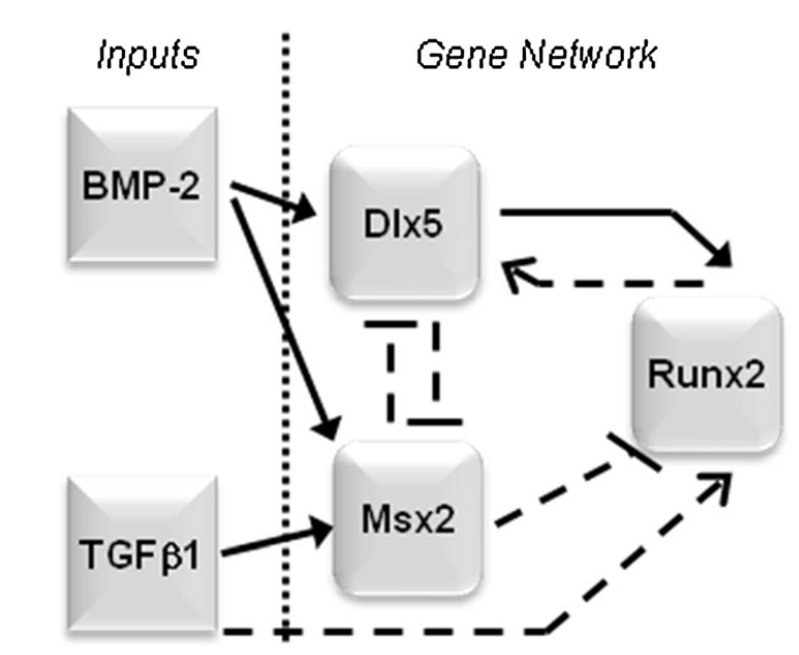
\includegraphics[scale=0.25]{regulatory_network.jpg}
	\caption{\label{GRNs} Potential regulatory networks derived from the literature, as noted in \cite{Kirkham}}
\end{figure} 

In order to identify which of the GRNs in \hyperref[GRNs]{figure 1} yield stable models that correspond to the expression profiles (see \hyperref[table1]{figure 2}), the author did some experiments with simple Java programs.

\begin{figure}[!htb]
  \centering
  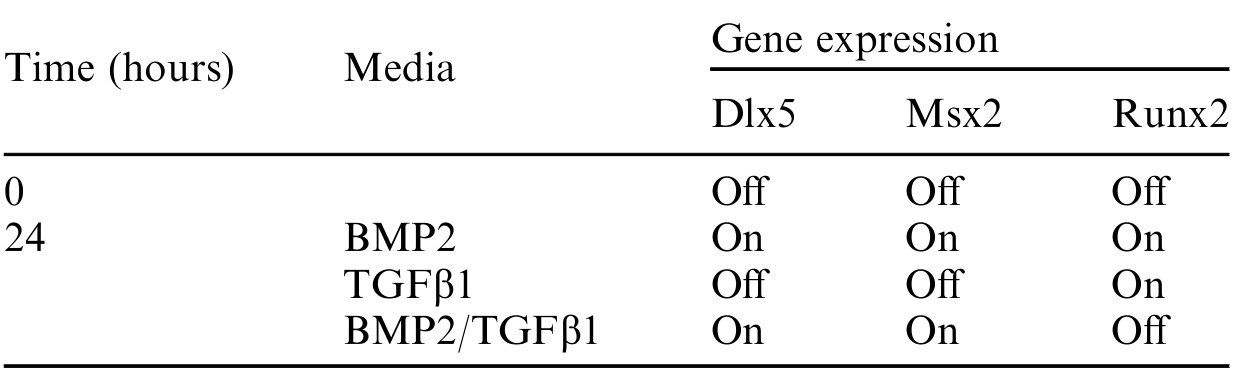
\includegraphics[scale=0.25]{table1.jpg} 
  \caption{\label{table1} (experimentally) measured expression profiles of species Dlx5, Msx2 and Runx2 in media BMP2, TGF$\beta1$ and BMP2 as well as TGF$\beta1$ at the initial time and after 1 day (source: \cite{Kirkham})}
\end{figure}

The preliminary studies of the authors led to the suspicion that the (adoption of the) methodology sketched in \cite{Kirkham} is not quite consistent with the data presented in \hyperref[table1]{figure 2}. 
Thus, the author wrote a program for a systematic study how many of the potential GRNs are consistent with the expression table in \cite{Kirkham}.

Of the $3^{5}=243$ potential GRNs in \hyperref[GRNs]{figure 1}, \cite{Kirkham} identified three that were stable and that corresponded to the expression data. The program the author wrote (which can be found in \hyperref[AppendixB]{Appendix B}) however found not a single one (indicated however that 24 (respective 36 with disjunctive logical connection) of these were not stable). 

To get a more comprehensive understanding of the methodology employed in \cite{Kirkham}, in the second step, a fixed point analysis of the fitting model identified in the paper was performed. Since the methodology was not entirely clear from the paper, different assumptions were tested based on the models identified by \cite{Kirkham}.

\subsubsection{Fixed point analysis of reported networks} \label{sssec:FPanalysis}
Since the process discussed in \ref{sssec:BMidentification} yielded results inconsistent with the results discussed in \cite{Kirkham}, the logical step seemed to be a fixed point analysis of these GRNs.

As \cite{Kirkham} reported that the only stable GRNs consistent with the (qualitative) expression profile measured (see \hyperref[table1]{figure 2}) were the GRNs where the influence of TGF$\beta1$ and Msx2 on Runx2, as well of Dlx5 on Msx2 were inhibitory and the influence of Msx2 on Dlx5 was activitory, a fixed point analysis was only done for the GRNs depicted in \hyperref[FPGRNs]{figure 3}.

\begin{figure}[!htb]
  \centering
  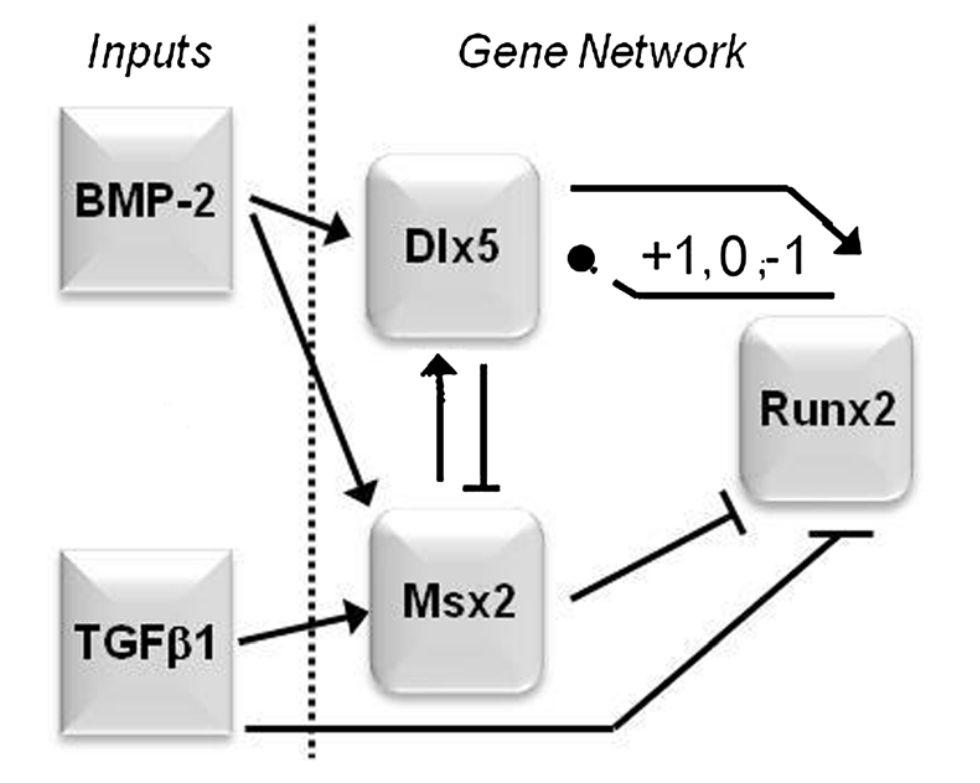
\includegraphics[scale=0.25]{regulatory_network_results.jpg} 	  	
  \caption{\label{FPGRNs} regulatory networks fitting expression profiles (source: \cite{Kirkham})}
\end{figure}

Based on the inconsistency of the results of the first step sketched in \ref{sssec:BMidentification} with \cite{Kirkham}, and the fact that the latter was not very clear about their assumptions, the goal of the fixed point analysis was to reconstruct the BMs used in the paper. 

Since it was not entirely clear whether the logical connection in the boolean expression was disjunctive or conjunctive, as well as how the absence of a GF in the medium was modelled in the boolean expression, different combinations were tried out for the fixed point analysis with the hope to derive which boolean expressions \cite{Kirkham} was based upon.

In the following, a fixed point analysis based on \hyperref[FPGRNs]{figure 3} will be performed, where the influence of Runx2 on Dlx5 will be activatory (case 1), inhibitory (case 2) or no influence of Runx2 on Dlx5 will be assumed (case 3).
Each case itself will contain three subcase specifying the environment (x.1: only BMP2 present, x.2: only TGF$\beta$1 present, x.3: BMP2 as well as TGF$\beta$1 present).

Since \cite{Kirkham} is not explicit on whether the boolean expressions are linked by conjunctions or disjunctions, both cases will be investigated, and in the best case the results will indicate whether the junction is conjunctive or disjunctive.

Due to the large number of cases these missing assumptions generate, the 36 fixpoint analyses can be found in the appendix (\hyperref[AppendixC]{Appendix C}). \\

An analysis of these cases shows that none of the assumptions are consistent with the boolean networks reported in \cite{Kirkham}. For the case where only TGF$\beta$1 is present, none of the assumptions generate a steady state where both Dlx5 and Msx2 are not expressed and Runx2 is expressed.

This expression pattern is unexpected for the regulatory networks depicted in \hyperref[FPGRNs]{figure 3} since TGF$\beta$1 has an inhibitory effect on Runx2 and thus the expression of Runx2 would only be expected with an expression of Dlx5. 
\hyperref[table1]{figure 2} however shows that a low expression of Dlx5 was measured. 
Thus this regulatory network seemed surprising to the intuition of the author. \\

The case of the GRN with the presence of TGF$\beta$1 however is not the only case when the steady state of the boolean network does not correspond to the reported expression profile.
In the case of the influence of Runx2 on Dlx5 to be activatory and both GFs to be present, none of the assumptions reproduce the GRNs measured behaviour that both Dlx5 and Msx2 are expressed but Runx2 is not. 

This case seems a little more intuitive; however if a conjunctive connection of the expressions in the boolean terms is assumed, only expression of Msx2 is reached (since Dlx5 will not be expressed as Runx2 is not expressed). If a disjunctive connection in the boolean terms is assumed, all three species will be expressed (since Runx2 will be expressed when Dlx5 is expressed). \\

In the case of inhibitory or no influence of Runx2 on Dlx5 with the presence of both GFs, an oscillation is observed for the conjunctive case. This occurs since the expression of Msx2 leads to the expression of Dlx5, which however leads to the inhibition of the expression of Msx2. With the lack of expression of Msx2, Dlx5 will not be expressed anymore and not inhibit the expression of Msx2 anymore, leading to it being expressed again.

\hyperref[table1]{figure 2} however sees the expression of both species as a steady state.

\subsection{Odefying Kirkham} \label{ssec:Odefyinvest}
Contrary to \ref{ssec:BMinvest}, this subsection will discuss the attempt at reconstructing the results presented in \cite{Kirkham} through the use of the Odefy 1.19 toolbox in \href{https://www.gnu.org/software/octave/}{GNU Octave}
4.0.2. Since Odefy was written for octave 3.x, some minor changes to the software were necessary (see \ref{sssec:ChangesOdefy}).

In order to follow the workflow of the study, first the candidate networks depicted in \hyperref[GRNs]{figure 1} were created. Subsequently the corresponding continuous models were created (\hyperref[sssec:Modelcreation]{Appendix D}), before their behaviour over time was simulated (\hyperref[sssec:simulationCM]{Appendix D}).

For the interesting case \cite{Kirkham} reports (that conforms to their measured data), a more extensive case study is done in \ref{sssec:Casestudy}, whose results will be discussed in \ref{sssec:Discussioncasestudy}.

\subsubsection{Odefy}
\href{http://www.helmholtz-muenchen.de/icb/software/odefy/index.html}{Odefy}, a MATLAB and GNU Octave compatible toolbox for the "odefication" (transformation into continous ODEs) of boolean models, has been developed by the \href{http://www.helmholtz-muenchen.de/icb/index.html}{Institute for Computational Biology of the Helmholtz-
Zentrum M{\"u}nchen}.

As noted in \ref{sssec:Motivationkirkham}, ODEs allow for a more detailled and quantitative characterization of GRNs. Qualitative (biological) knowledge is represented as BMs, which are transformed into continuous model, that are fitted with quantitative data (for a sketch of the workflow see \hyperref[odefy_workflow]{figure 4}).

Odefy uses the HillCube modeling technique. With $\overline{B}_{i}$ as the HillCube model of $\overline{x}_{i}$, the following differential equation is reached: $\dot{\overline{x}}_{i} = \frac{1}{\tau_{i}} (\overline{B}_{i} (\overline{x}_{i_{1}}, \overline{x}_{i_{2}},..., \overline{x}_{i_{N_{i}}} ) - \overline{x}_{i} )$, where $\tau_{i}$ stands for the lifespan of species $X_{i}$ (as described in \ref{ssec:prop}).

\begin{figure}[!hbt]
  \centering
  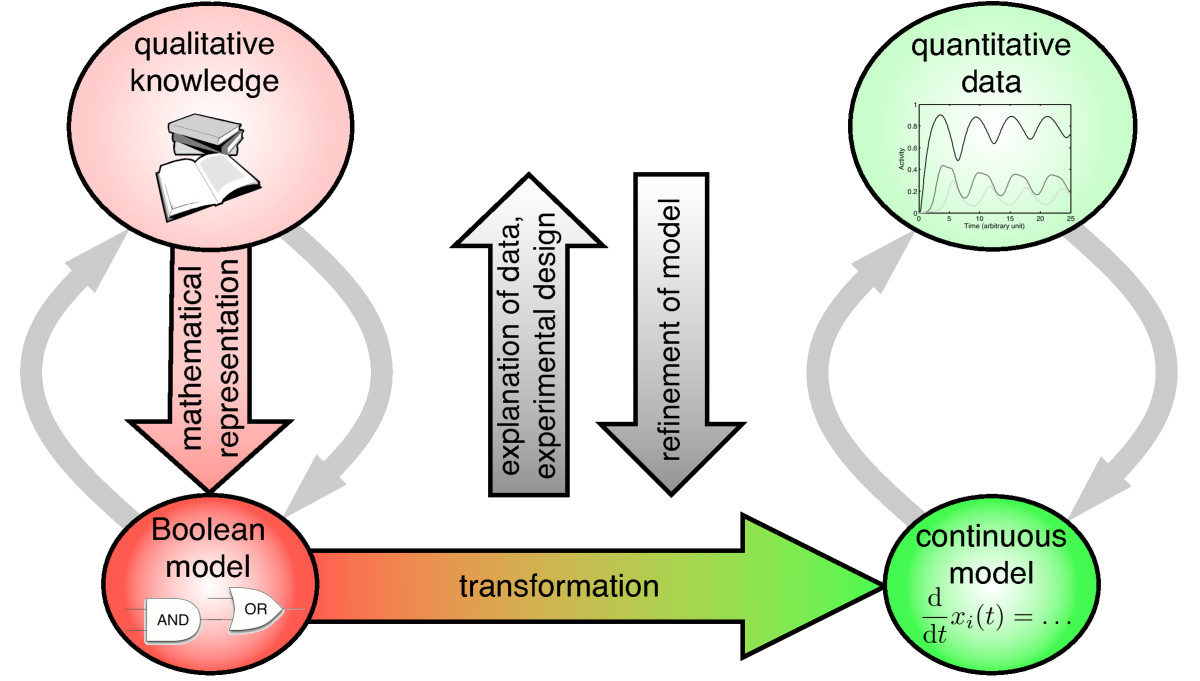
\includegraphics[width=0.8\textwidth]{odefy.jpg}
  \caption{\label{odefy_workflow} Sketch of the odefy workflow.}
\end{figure}


\subsubsection{Practical approach to Odefy} \label{sssec:Pracapproach}
In Odefy, the boolean models are specified as a set of strings describing the influences of other species onto the species specified.
The semantics of these strings of the form \textit{LHS = RHS} is that LHS is considered 'on' iff RHS is true, and 'off' otherwise.

The candidate BMs discussed in \cite{Kirkham}, as derived from the literature (see also \hyperref[GRNs]{figure 1}), use the GFs
BMP2 and TGF$\beta$1, as well as the genes Dlx5, Msx2 and Runx2.
Since the authors assumed that the influence of TGF$\beta$1 to Msx2, BMP2 to Msx2 and Dlx5, as well as the influence of Dlx5 on Runx2 was activatory, the following substrings are fixed in the model description (odefy-syntax):

'Msx2 = TGF$\beta1$ $\&\&$ MBP2'\footnote{As discussed in \ref{ssec:BMinvest} it is not quite clear whether the junction of the species is a conjunction or a disjunction. In the spirit of \ref{ssec:Formaldescription} in this investigation a conjunction is used.}, 'Dlx5 = BMP2', 'Runx2 = Dlx5' 

The approach in this course work is two-fold; it generates the potential candidate networks as noted in \hyperref[GRNs]{figure 1} and performs simulations of (hill-cube) continuous homologue. Due to the large number of resulting networks ($2*3^{5}$), the results will not be discussed here, and can be found in \ref{AppendixD}.
This section will instead focus on the reduced set of candidate networks in \cite{Kirkham}, where the influence of TGF$\beta$1 and Msx2 on Runx2 is inhibitory, the influence of Msx2 on Dlx5 is excitatory and the influence of Dlx5 on Msx2 is inhibitory (see \hyperref[FPGRNs]{figure 3}).

However, with the three growth media, two possible logical connections and three candidate networks, only a representative case (where Runx2 regulates Dlx5 negatively\footnote{The case that \cite{Kirkham} identifies as matching the experimentally observed oscillation behaviour}) is presented in the following.

\subsubsection{Case study: negative regulation of Runx2 on Dlx5} \label{sssec:Casestudy}
As mentioned in \ref{sssec:Pracapproach}, this case study will sketch the process from the boolean model to the continuous expression profile for the regulatory network where Runx2 regulates Dlx5 negatively.

As the boolean model is specified as a boolean expression, a boolean expression for the corresponding network is specified by
\begin{lstlisting}
Runx2Dlx5Inhibitory_and = {
	'BMP2 = <>', 
	'TGFb1 = <>', 
	'Dlx5 = Msx2 && ~Runx2 && BMP2', 
	'Msx2 = BMP2 && TGFb1 && ~Dlx5', 
	'Runx2 = Dlx5 && ~Msx2 && ~TGFb1'
}
\end{lstlisting}
for the case that the logical connection is a conjunction, and 
\begin{lstlisting}
Runx2Dlx5Inhibitory_or = {
	'BMP2 = <>', 
	'TGFb1 = <>', 
	'Dlx5 = Msx2 || ~Runx2 || BMP2', 
	'Msx2 = BMP2 || TGFb1 || ~Dlx5', 
	'Runx2 = Dlx5 || ~Msx2 || ~TGFb1'
}
\end{lstlisting}
for the case the logical connection is a disjunction.

The corresponding boolean models and the structs needed for the simulation by Odefy are constructed as follows:
\begin{lstlisting}
model_and = ExpressionsToOdefy(Runx2Dlx5Inhibitory_and)
simstruct_and = CreateSimstruct(model_and)
simstruct_and.type = 'hillcube'
model_or = ExpressionsToOdefy(Runx2Dlx5Inhibitory_or)
simstruct_or = CreateSimstruct(model_or)
simstruct_or.type = 'hillcube'
\end{lstlisting}
under the usage of the HillCube method as discusssed in \ref{sssec:Hillcube}.

Since in both cases, the expression of the genes under investigation was considered off at the beginning of the simulation\footnote{Since as \cite{Kirkham} notes, mRNA levels are low in mouse embryonic stem cells}, the initial values for these species was set to 0:
\begin{lstlisting}
simstruct_and = SetInitialValue(simstruct_and, 'Dlx5', 0)
simstruct_and = SetInitialValue(simstruct_and, 'Msx2', 0)
simstruct_and = SetInitialValue(simstruct_and, 'Runx2', 0)
simstruct_or = SetInitialValue(simstruct_or, 'Dlx5', 0)
simstruct_or = SetInitialValue(simstruct_or, 'Msx2', 0)
simstruct_or = SetInitialValue(simstruct_or, 'Runx2', 0)
\end{lstlisting}

For the individual cases (presence of media / logical connection in boolean expression), the following results were obtained:

\paragraph{BMP2 only with conjunction}
With this setup, the following code is executed:
\begin{lstlisting}
simstruct_and = SetInitialValue(simstruct_and, 'BMP2', 1)
simstruct_and = SetInitialValue(simstruct_and, 'TGFb1', 0)
[t,y] = OdefySimulation(simstruct_and, 0, 0);
plot(t,y, {".", ".", 'd', '*', 'p'}, "markersize", 2);
legend(simstruct_and.model.species);
xlabel("time");
ylabel("expression");
title("Runx2->Dlx5 inhibitory, BMP2 only, conjunction");
axis([0, 10, -0.1, 1.1]);
\end{lstlisting}
The simulation yields a static behaviour where no dynamic is visible (as can be seen in \hyperref[firstCase]{figure 5})
%
\begin{figure}[!htb]
	\centering
	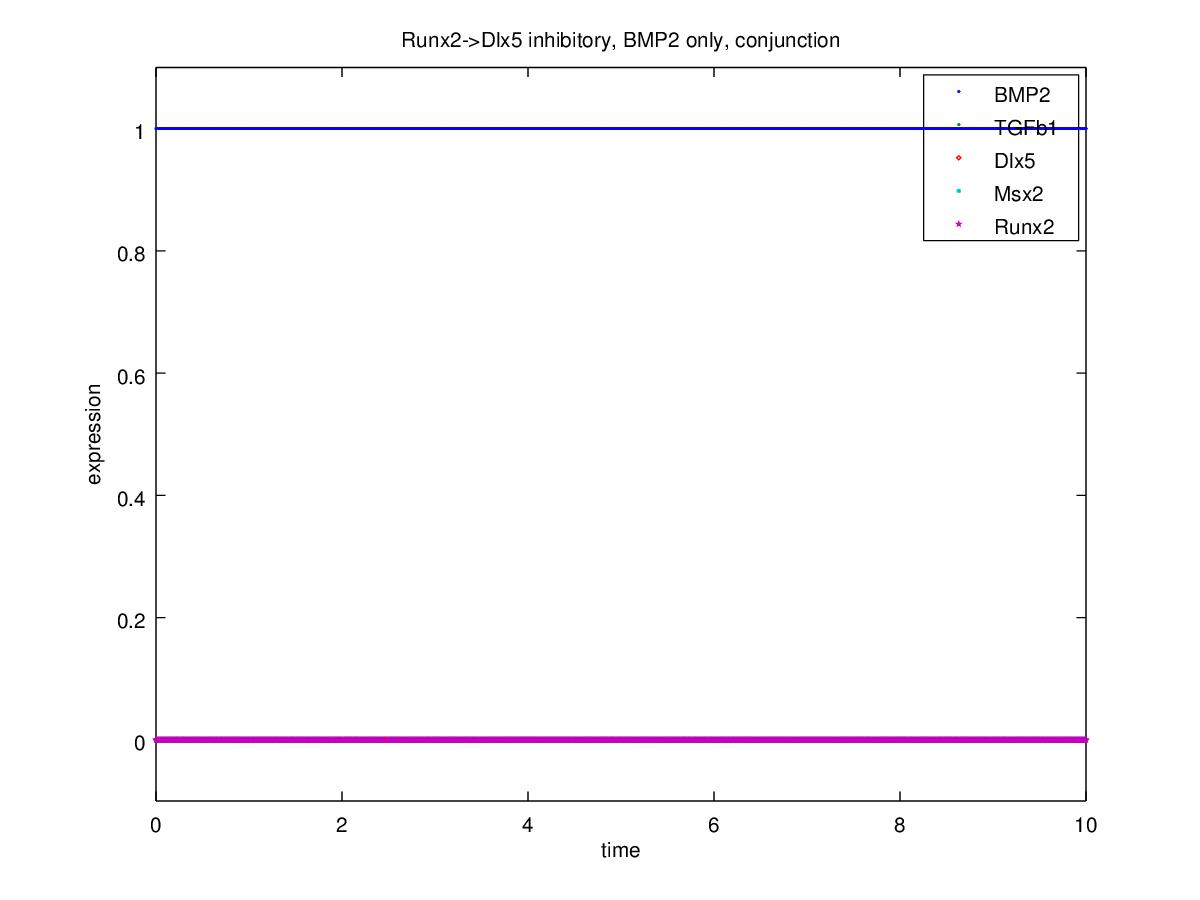
\includegraphics[scale=0.55]{case1.jpg}
	\caption{\label{firstCase} conjunctive logical connection of boolean expressions with the presence of the GF BMP2}
\end{figure}

\paragraph{TGFb1 only with conjunction}
With this setup, the following code is executed:
\begin{lstlisting}
simstruct_and = SetInitialValue(simstruct_and, 'BMP2', 0)
simstruct_and = SetInitialValue(simstruct_and, 'TGFb1', 1)
[t,y] = OdefySimulation(simstruct_and, 0, 0);
plot(t,y, {".", ".", 'd', '*', 'p'}, "markersize", 2);
legend(simstruct_and.model.species);
xlabel("time");
ylabel("expression");
title("Runx2->Dlx5 inhibitory, TGFb1 only, conjunction");
axis([0, 10, -0.1, 1.1]);
\end{lstlisting}
The simulation yields a static behaviour where no dynamic is visible (as can be seen in \hyperref[secondCase]{figure 6})

\begin{figure}[!htb]
	\centering
	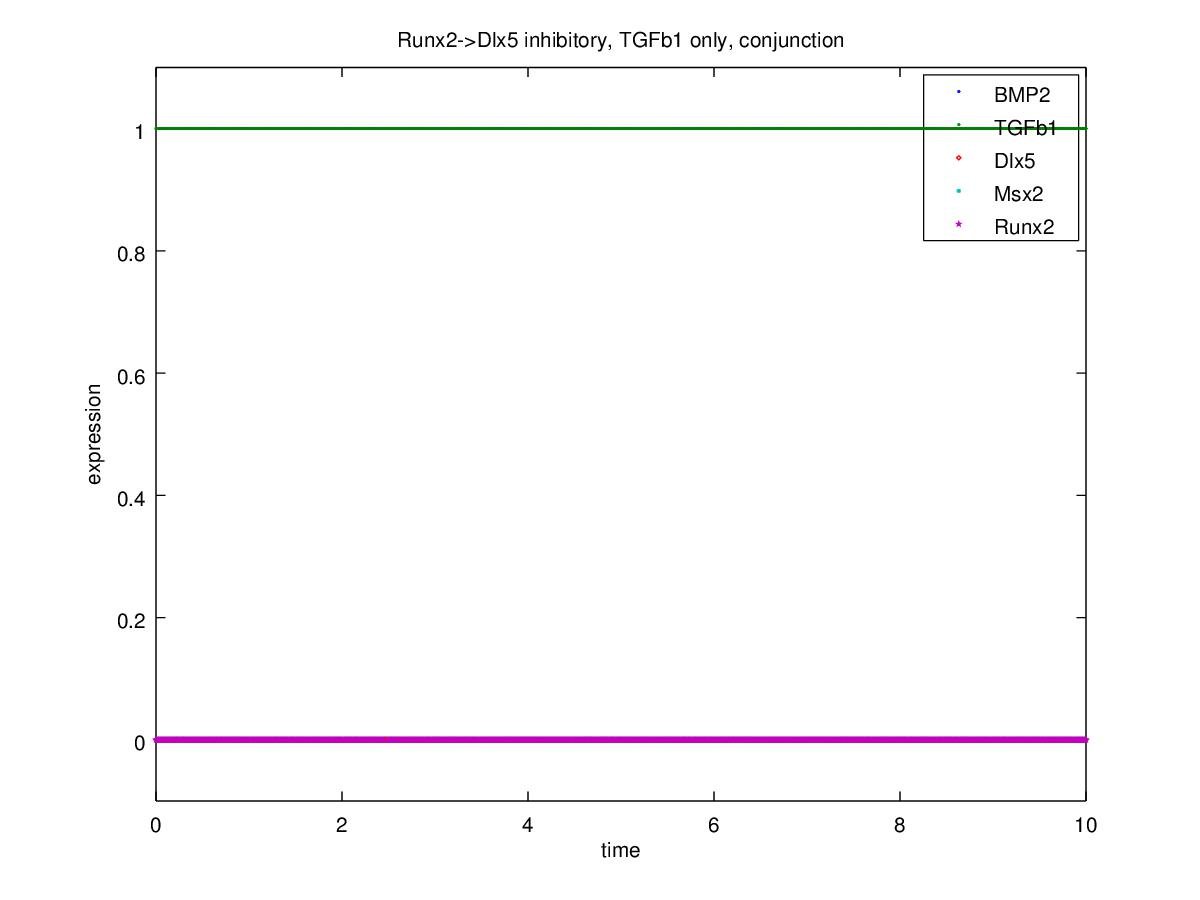
\includegraphics[scale=0.55]{case2.jpg}
	\caption{\label{secondCase} conjunctive logical connection of boolean expressions with the presence of the GF TGFb1}
\end{figure}

\paragraph{TGFb1 and BMP2 with conjunction}
With this setup, the following code is executed:
\begin{lstlisting}
simstruct_and = SetInitialValue(simstruct_and, 'BMP2', 1)
simstruct_and = SetInitialValue(simstruct_and, 'TGFb1', 1)
[t,y] = OdefySimulation(simstruct_and, 0, 0);
plot(t,y, {".", ".", 'd', '*', 'p'}, "markersize", 2);
legend(simstruct_and.model.species);
xlabel("time");
ylabel("expression");
title("Runx2->Dlx5 inhibitory, TGFb1 and BMP2, conjunction");
axis([0, 10, -0.1, 1.1]);
\end{lstlisting}
With the presence of both growth factors, dynamics can be observed in all three species (as can be seen in \hyperref[thirdCase]{figure 7}).
The activity of Runx2 is negligibly small; the expression levels of Dlx5 and Msx2 however express a clear dynamic after some (rudimentary) transient oscillation, when they stabilize at roughly half the maximal expression level.

\begin{figure}[!htb]
	\centering
	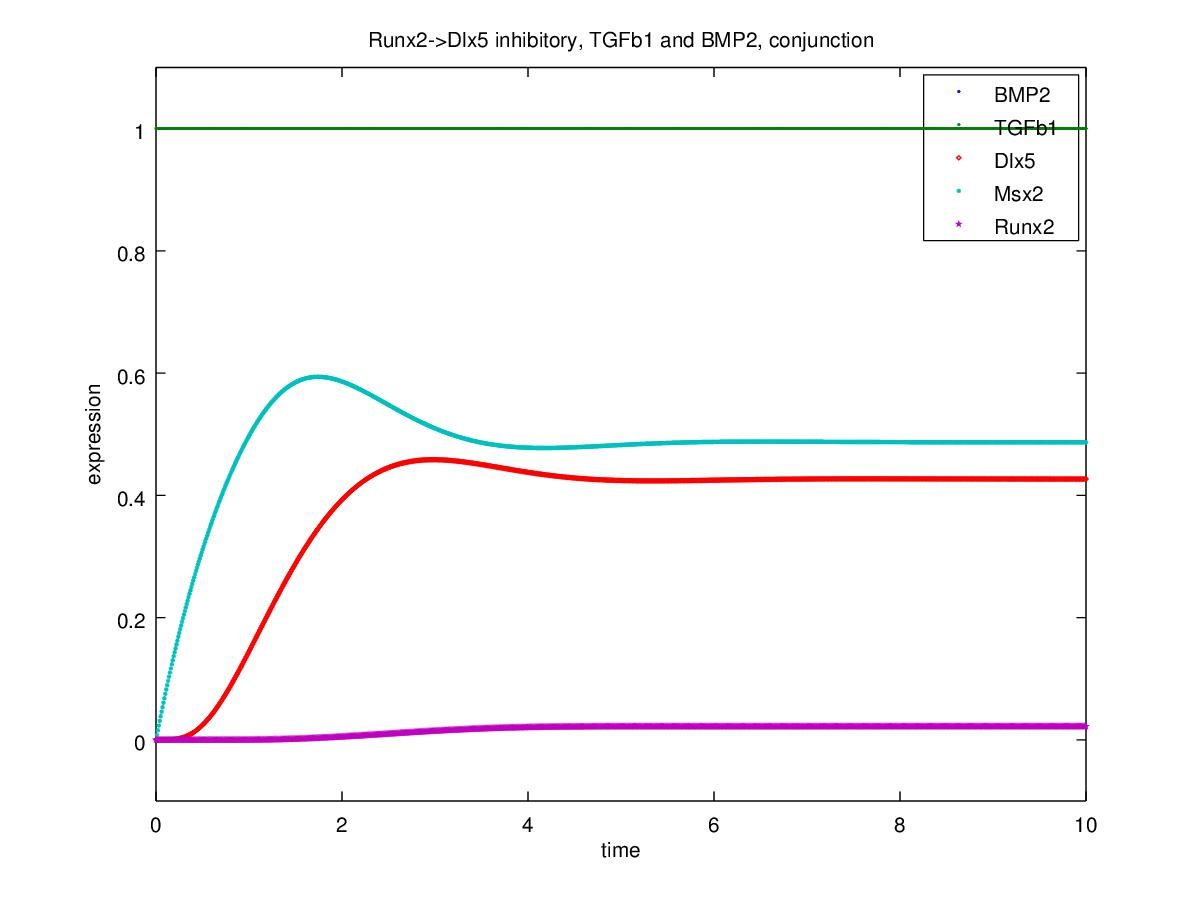
\includegraphics[scale=0.55]{case3.jpg}
	\caption{\label{thirdCase} conjunctive logical connection of boolean expressions with the presence of both GFs}
\end{figure}

\paragraph{BMP2 with disjunction}
With this setup, the following code is executed:
\begin{lstlisting}
simstruct_or = SetInitialValue(simstruct_or, 'BMP2', 1)
simstruct_or = SetInitialValue(simstruct_or, 'TGFb1', 0)
[t,y] = OdefySimulation(simstruct_or, 0, 0);
plot(t,y, {".", ".", 'd', '*', 'p'}, "markersize", 2);
legend(simstruct_or.model.species);
xlabel("time");
ylabel("expression");
title("Runx2->Dlx5 inhibitory, BMP2 only, disjunction");
axis([0, 10, -0.1, 1.1]);
\end{lstlisting}
In the case of disjunctive logical connection in the boolean expression and the presence of the GF BMP2, the species exhibit a monotonous increase in concentration with seemingly logarithmic growth (see \hyperref[fourthCase]{figure 8}). Although the different species exhibit similar qualitative behaviour, a clear difference in expression levels can be seen between the species with expression levels of Msx2 relatively low compared to the other two species and only Runx2 being completely expressed.

\begin{figure}[!htb]
	\centering
	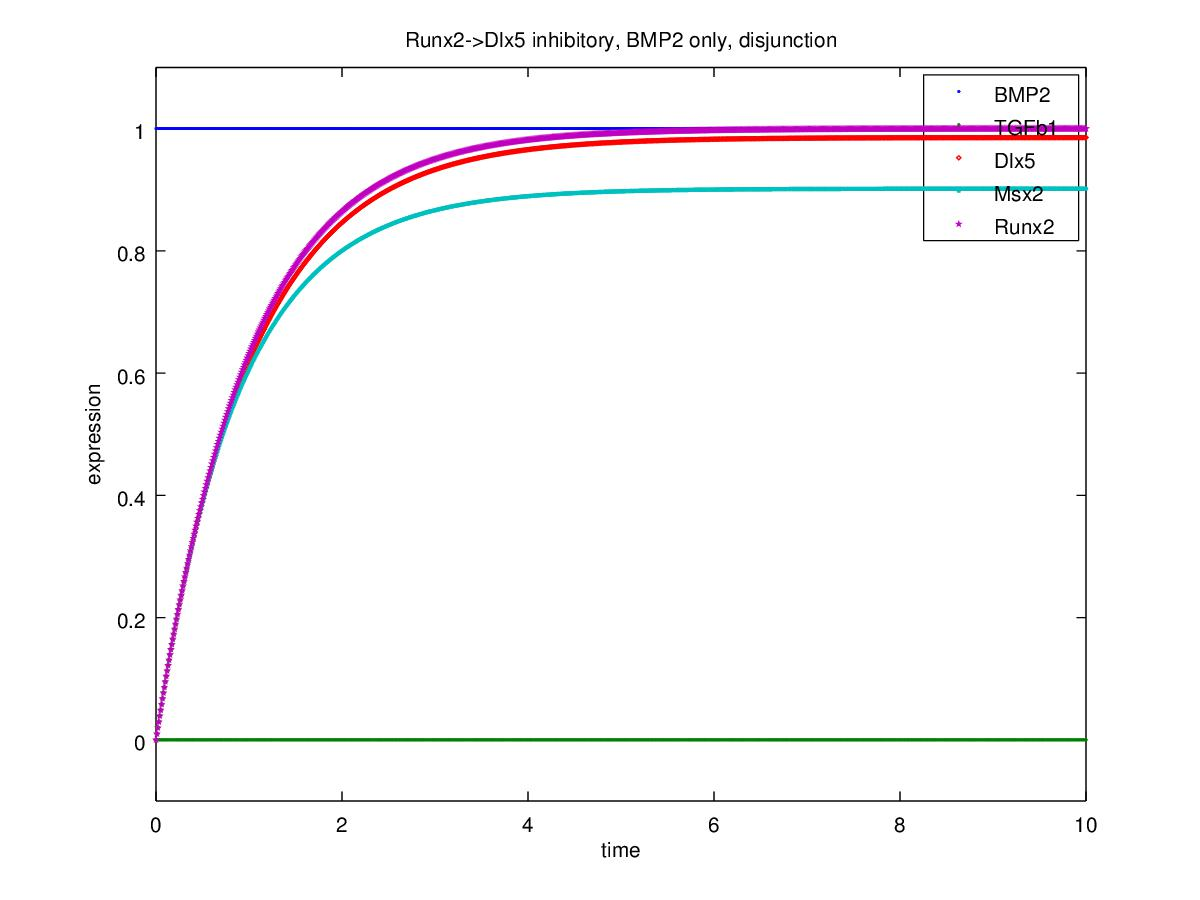
\includegraphics[scale=0.55]{case4.jpg}
	\caption{\label{fourthCase} disjunctive logical connection of boolean expressions with the presence of BMP2}
\end{figure}

\paragraph{TGFb1 with disjunction}
With this setup, the following code is executed:
\begin{lstlisting}
simstruct_or = SetInitialValue(simstruct_or, 'BMP2', 0)
simstruct_or = SetInitialValue(simstruct_or, 'TGFb1', 1)
[t,y] = OdefySimulation(simstruct_or, 0, 0);
plot(t,y, {".", ".", 'd', '*', 'p'}, "markersize", 2);
legend(simstruct_or.model.species);
xlabel("time");
ylabel("expression");
title("Runx2->Dlx5 inhibitory, TGFb1 only, disjunction");
axis([0, 10, -0.1, 1.1]);
\end{lstlisting}
The disjunctive BM with the presence of TGF$\beta$1 exhibits a similar behaviour as the medium of BMP2 with a monotonous increase in expression levels with seemingly logarithmic growth (see \hyperref[fifthCase]{figure 9}). In contrast to the medium with BMP2 however, the expression levels differ. In this medium, the expression of Msx2 is the strongest of the three, and the other two species (Dlx5 and Runx2) are comparatively weekly expressed.

\begin{figure}[!htb]
	\centering
	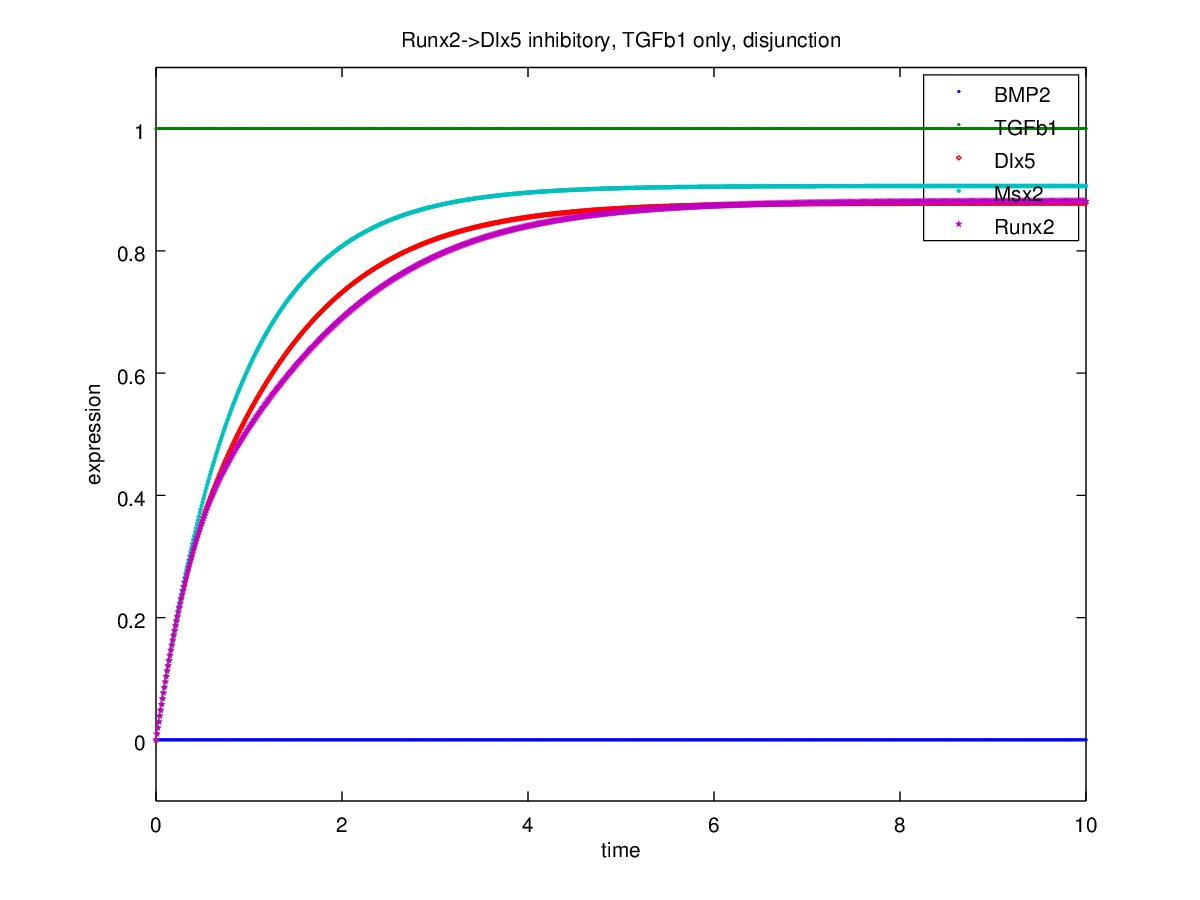
\includegraphics[scale=0.55]{case5.jpg}
	\caption{\label{fifthCase} disjunctive logical connection of boolean expressions with the presence of TGFb1}
\end{figure}

\paragraph{Both media with disjunction}
With this setup, the following code is executed:
\begin{lstlisting}
simstruct_or = SetInitialValue(simstruct_or, 'BMP2', 1)
simstruct_or = SetInitialValue(simstruct_or, 'TGFb1', 1)
[t,y] = OdefySimulation(simstruct_or, 0, 0);
plot(t,y, {".", ".", 'd', '*', 'p'}, "markersize", 2);
legend(simstruct_or.model.species);
xlabel("time");
ylabel("expression");
title("Runx2->Dlx5 inhibitory, TGFb1 and BMP2, disjunction");
axis([0, 10, -0.1, 1.1]);
\end{lstlisting}
The disjunctive BM with the presence of both media exhibits a similar behaviour as the individual media. All species exhibit a monotonous increase in expression levels with seemingly logarithmic growth (see \hyperref[sixthCase]{figure 10}). In this scenario, the expression of Runx2 is visibly weaker than the expression of Dlx5 and Msx2, which exhibit a very similar behaviour approaching almost full expression before they stagnate.

\begin{figure}[!htb]
	\centering
	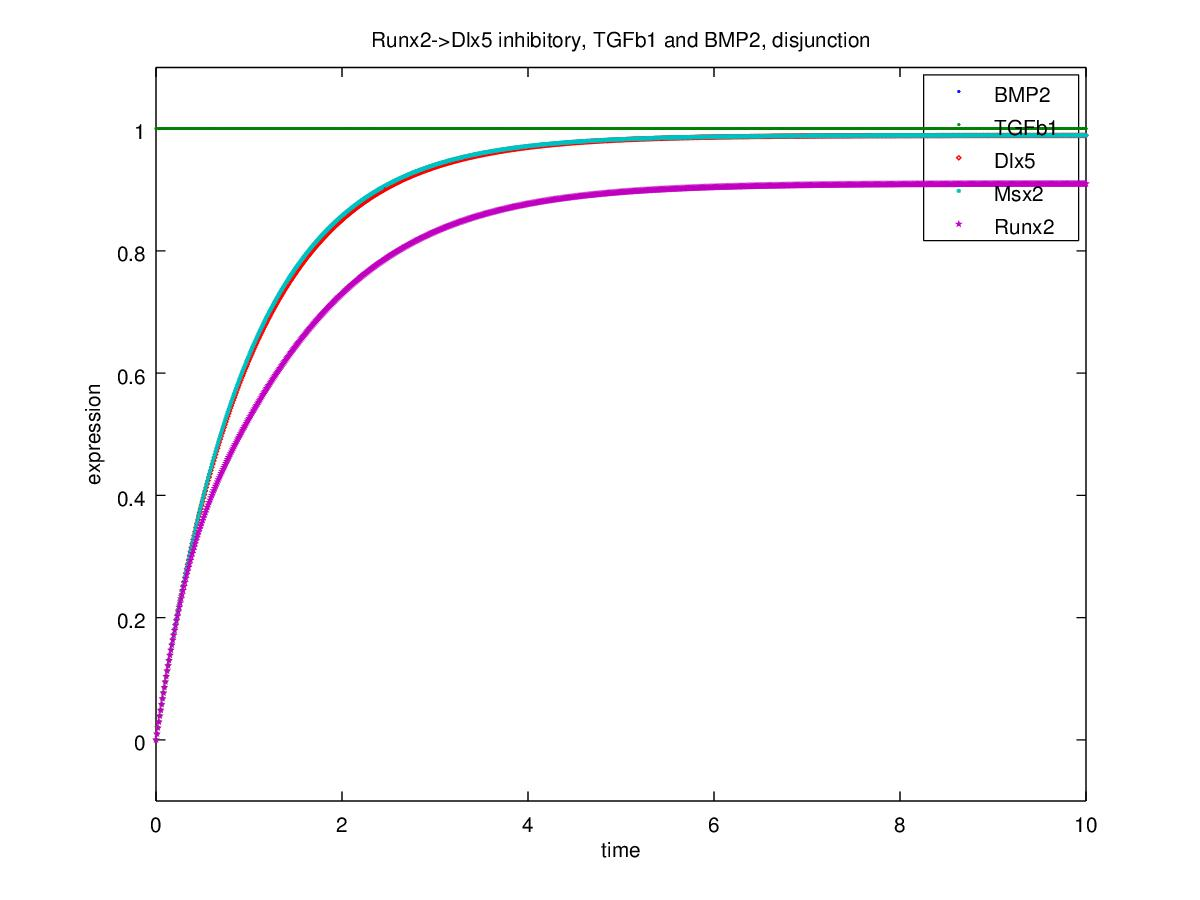
\includegraphics[scale=0.55]{case6.jpg}
	\caption{\label{sixthCase} disjunctive logical connection of boolean expressions with the presence of TGFb1 and BMP2}
\end{figure}

\subsubsection{Discussion of case study} \label{sssec:Discussioncasestudy}
The case study (\ref{sssec:Casestudy}) shows very clear differences in the expression profiles under the assumption of the logical connection within the boolean expression.
The intuition that led to the investigation of the different connections and the resulting behaviour in the perfect homologues of the boolean models thus seems to be confirmed.

The qualitative behaviour of the expression profiles with the logical disjunction shows a clear increase in expression for all three species in all three media. Comparing this behaviour to the behaviour discussed in \cite{Kirkham} however, shows that the logical connection employed in this was clearly not the disjunction, since with the presence of both media an oscillatory behaviour should be observed, and in the presence of just one media, the expression of all three species is expected to very quickly reach a stable level.
With the behaviour reported in \ref{sssec:Casestudy} for the disjunction however, a continuous increase of all three species is observed for all three media, describing a very different behaviour. It can thus be assumed that the disjunction was not the logical connection of choice for \cite{Kirkham}. \\

The first three cases reported in \ref{sssec:Casestudy} (in which a conjunction was employed in the boolean expressions) however are more interesting, since a more varied and qualitatively similar behaviour to \cite{Kirkham} was observed.
In the presence of only one of the GFs the (conjunctive) perfect homologue shows stationary behaviour, similar to the (qualitative) behaviour in \cite{Kirkham}; however in their data, transient oscillations (as short as they may be) are present, whereas in this course work, these weren't reproducible. 
In the case of the presence of both GFs however, the differences are even more pronounced; Although some (slight) oscillatory behaviour can be observed in \hyperref[thirdCase]{figure 7} for Dlx5 and Msx2, this behaviour seems more like transient oscillations than proper oscillations (for all three species), as reported in \cite{Kirkham}. \\

In summary, it can be said that although some tendencies of the desired behaviour were reproduced in this course work, this course work failed to reproduce the behaviour reported in \cite{Kirkham}.
However, these investigations illuminated the question whether a conjunctive or disjunctive logical connection was used for the boolean model in \cite{Kirkham}.


\subsubsection{Practical aspects Odefy} \label{sssec:ChangesOdefy}
Since Odefy 1.19 (at the time of writing the most current version of the odefy toolbox) was written with GNU Octave 3.x in mind, a few minor changes were necessary in order to make the toolbox work for Octave 4.0.2 (at the time of writing the most current version of GNU octave). 

The author chose to include the current version of Octave in the setup, since he assumes that most (future) readers will use this version, and the following paragraphs would enable them to reproduce the discussed results as well as continue using Odefy (unless a future release of Odefy will take these into account). \\

The (minor) changes are as follows:
\\
\textbf{code/simulation/OdefySimulation.m}: \\
The \textit{extname} must not be in the \textit{cmd} variable, thus line 80 needs to be changed to:
\begin{lstlisting}
cmd = sprintf('yp = lsode(@(t,y)%s(y,t,simparams), 
simstruct.initial'', realtime);',tmpname);
\end{lstlisting}

\textbf{code/models/validvarname.m}:

Another condition to set \textit{isvalid} to 0 must be included (appended in line 16):
\begin{lstlisting}
if numel(regexp('ydw', '[^A-Za-z_0-9]'))>0
    isvalid=0;
end
\end{lstlisting}

The behaviour for replacing invalid characters by underscore need to be modified. As such lines 27-32 need to be replaced by:
\begin{lstlisting}
varname=regexprep('ydw*?', '[^A-Za-z_0-9]', '_');
\end{lstlisting}

\section{Discussion} \label{sec:Discussion}
The paper analyzed in this course work employed a promising approach to identifying gene regulatory networks from a modelling perspective. 

It was light on the mathematical background, which could be found easily (and well elaborated) in the papers \cite{Krumsiek} and \cite{Wittmann}.

Its brevity on the employed methodology however has shown to lead to numerous challenges in reproducing the results reported. 
Avoiding to state the assumptions the boolean models are based upon have led to a large number of cases and variations identified in \ref{sssec:FPanalysis}.

However, even with the large number of cases or possible combinations of assumptions, no consistent results on the BM used in \cite{Kirkham} could be found. \\

None of the BM reported to be consistent with the expression profiles listed in \hyperref[table1]{figure 2} were confirmed in \ref{sssec:FPanalysis}, despite testing a rather large set of assumptions. This indicates that either the methodology used in the paper was not reported sufficiently or the inconsistencies arising during the research were resolved differently than in this course work.
Most certainly the author does not want imply that the discrepancies to \cite{Kirkham} couldn't be attributed to his lack of background in this field, and would most humbly request for clarification in methodology. \\

The oscillatory behaviour of the GRN reported by \cite{Kirkham} to be consistent with the data reported in \hyperref[table1]{figure 2} was not originally meant to be part of this course work. However, due to the inconclusiveness of \ref{sssec:FPanalysis}, the author hoped to gain an insight into the formulation of the boolean expressions used in \cite{Kirkham}.
Despite some major differences in the behaviour after transient oscillation, this comparison implies that the logical connection in the boolean expressions were the conjunction (which is consistent with \hyperref[ssec:Formaldescription]{Appendix A}). \\

Resumptively, although intrigued by the approach sketched in \cite{Wittmann} and \cite{Krumsiek}, the author does not share the intuition that boolean models are suited to describe the behaviour of GRNs in more general contexts, and has not yet been convinced that they are suited for the research described here. 
Although interesting and promising, the author is left sceptical of the results presented in \cite{Kirkham}, which however could be due to his lack of training in its methodology. \\

Despite the broad approach taken in this course work, no results consistent with \cite{Kirkham} could be achieved, and not even a clear result could be formulated as to what assumptions the boolean models investigated in \cite{Kirkham} were based upon.

\begin{appendices}
\section*{Appendix A: Boolean models} \label{AppendixA}
This appendix will describe the propaedeutic aspects of boolean models not discussed in the course work.

As mentioned in \ref{sec:Theory}, Boolean models (BMs) express qualitative biological knowledge, meaning that a species is either active or inactive (binary state). Represented as a graph (see \hyperref[GRNs]{figure 1}), the species are seen as nodes, whereas the interactions between the species are modeled as edges (which can be either activating, inhibatory or no influence).
Despite their coarseness, BMs can reproduce the qualitative behaviour of biological systems.

Due to their discrete nature however, they are not suited for quantitative models. Thus they can neither explain nor predict quantitative experiments, which is increasingly important in systems biology. For these applications,
the transformation to systems of ordinary differential equations (ODEs) has shown to be fruitful.

\subsection*{Formal description} \label{ssec:Formaldescription}
Formally, boolean models for N species $X_{1}, X_{2},..., X_{N}$, represented by variables $x_{i} \in \{0, 1\}$, are
defined by a set of species $R_{i} := \{X_{i_{1}}, X_{i_{2}},..., X_{i_{N_{i}}}\} \subset
\{X_{1},...,X_{N}\}$ influencing $X_{i}$, as well as an update function $B_{i}: \{0, 1\}^{N_{i}} \rightarrow \{0, 1\}$ for every combination of ($x_{i_{1}},..., x_{i_{2}}, x_{i_{N_{i}}}) \in \{0, 1\}^{N_{i}}$.

Mapped on the (hyper-) unit cube, the nodes ($\xi_{i_{1}},\xi_{i_{2}},..., \xi_{i_{N_{i}}}) \in \{0, 1\}^{N_{i}}$ corresponding to the domain of $B_{i}$, can logically be interpreted as $( \bigwedge_{ij| \xi_{ij = 1}} x_{ij} ) \wedge ( \bigwedge_{ij| \xi_{ij = 0}} \neg x_{ij} )$, meaning that $B_{i}$ will be true for the nodes of the cube where
the coordinate equals the boolean value of influence of the activation function.
With the sum-of-product representation, $B_{i}$ can now be viewed as: $B_{i} (x_{i_{1}}, x_{i_{2}},..., x_{i_{N_{i}}} ) = \bigvee_{(\xi_{i_{1}}, \xi_{i_{2}},..., \xi_{i_{N_{i}}}) | B_{i} ( \xi_{i_{1}}, \xi_{i_{2}},..., \xi_{i_{N_{i}}}) = 1} $ [ $( \bigwedge_{ij | \xi_{ij = 1}} x_{ij}) \wedge ( \bigwedge _{ij | \xi_{ij = 0}}  \neg x_{ij} ) $].

Thus each product can be represented  as a hyperedge between the start nodes $ S \subset \{X_{i_{1}}, X_{i_{2}},..., X_{i_{N_{i}}}\}$ and the end node $X_{i}$, with each pair $(s, X_{i}), s \in S$ carrying a sign on whether it is noted as a factor $x_{ij}$ or $\neg x_{ij}$ in the BM.

\section*{Appendix B: Code identification of stable BMs} \label{AppendixB}
This appendix will list the code used to identify stable boolean models from the GRNs (see \ref{sssec:BMidentification}) proposed in \cite{Kirkham}.

\lstinputlisting[language=Java, breaklines=true]{Main.java}
\section*{Appendix C: Results fixed point analysis} \label{AppendixC}
This appendix will list the results of the fixed point analysis of the boolean models identified as stable by \cite{Kirkham}.

As noted in \ref{sssec:FPanalysis}, some assumptions were not explicitly stated in the aforementioned publication. In order to identify the assumptions their approach is based upon, a systematic investigation of these assumptions is performed in the following. 

The three models identified by \cite{Kirkham} are coded as the cases, where the influence of Runx2 on Dlx5 will be activatory (case 1), inhibitory (case 2) or no influence of Runx2 on Dlx5 will be assumed (case 3).
Each case itself will contain three subcase specifying the environment (x.1: only BMP2 present, x.2: only TGF$\beta$1 present, x.3: BMP2 as well as TGF$\beta$1 present).

Furthermore are the cases distinguished by whether the logical connection in the boolean models is conjunctive or disjunctive.

An additional assumption tested is whether in the absence of a growth factor (BMP2 / TGF$\beta$1), a constant 'Off' is assumed for this variable in the boolean model, or whether this variable is ignored.

The following 18 cases will assume that in the absence of a growth factor the variable will be considered \textit{Off}. \\

\textbf{case 1.1: Runx2 activatory on Dlx5, BMP2 only}: \\
\textit{conjunction:}
\\
\begin{tabular}{c c c c}
t & Dlx5 & Msx2 & Runx2 \\
\hline
0 & Off & Off & Off \\
1 & Off & Off & Off
\end{tabular}
\\
$\rightarrow$ A fixed point is reached no species being expressed.  
\\ \\
\textit{disjunction:}
\\ 
\begin{tabular}{c c c c}
t & Dlx5 & Msx2 & Runx2 \\
\hline
0 & Off & Off & Off \\
1 & On & On & On \\
2 & On & On & On
\end{tabular}
\\
$\rightarrow$ A fixed point is reached with all species being expressed
\\ \\
\textbf{case 1.2: Runx2 activatory on Dlx5, TGF$\beta1$ only}: \\
\textit{conjunction:}
\\ 
\begin{tabular}{c c c c}
t & Dlx5 & Msx2 & Runx2 \\
\hline
0 & Off & Off & Off \\
1 & Off & Off & Off
\end{tabular}
\\
$\rightarrow$ A fixed point is reached with no species being expressed.  
\\ \\
\textit{disjunction:}
\\ 
\begin{tabular}{c c c c}
t & Dlx5 & Msx2 & Runx2 \\
\hline
0 & Off & Off & Off \\
1 & Off & On & On \\
2 & On & On & Off \\
3 & On & On & On
\end{tabular}
\\
$\rightarrow$ A fixed point is reached with all species being expressed
\\ \\
\textbf{case 1.3: Runx2 activatory on Dlx5, BMP2 and TGF$\beta1$ present}: \\
\textit{conjunction:}
\\ 
\begin{tabular}{c c c c}
t & Dlx5 & Msx2 & Runx2 \\
\hline
0 & Off & Off & Off \\
1 & Off & On & Off \\
2 & Off & On & Off
\end{tabular}
\\
$\rightarrow$ A fixed point is reached with Msx2 being expressed.  
\\ \\
\textit{disjunction:}
\\ 
\begin{tabular}{c c c c}
t & Dlx5 & Msx2 & Runx2 \\
\hline
0 & Off & Off & Off \\
1 & On & On & On \\
2 & On & On & On
\end{tabular}
\\
$\rightarrow$ A fixed point is reached with all species being expressed
\\ \\
\textbf{case 2.1: Runx2 inhibitory on Dlx5, BMP2 only}: \\
\textit{conjunction:}
\\
\begin{tabular}{c c c c}
t & Dlx5 & Msx2 & Runx2 \\
\hline
0 & Off & Off & Off \\
1 & Off & Off & Off
\end{tabular}
\\
$\rightarrow$ A fixed point is reached no species being expressed.  
\\ \\
\textit{disjunction:}
\\ 
\begin{tabular}{c c c c}
t & Dlx5 & Msx2 & Runx2 \\
\hline
0 & Off & Off & Off \\
1 & On & On & On \\
2 & On & On & On
\end{tabular}
\\
$\rightarrow$ A fixed point is reached with all species being expressed
\\ \\
\textbf{case 2.2: Runx2 inhibitory on Dlx5, TGF$\beta1$ only}: \\
\textit{conjunction:}
\\ 
\begin{tabular}{c c c c}
t & Dlx5 & Msx2 & Runx2 \\
\hline
0 & Off & Off & Off \\
1 & Off & Off & Off
\end{tabular}
\\
$\rightarrow$ A fixed point is reached with no species being expressed.  
\\ \\
\textit{disjunction:}
\\ 
\begin{tabular}{c c c c}
t & Dlx5 & Msx2 & Runx2 \\
\hline
0 & Off & Off & Off \\
1 & On & On & On \\
2 & On & On & On \\
\end{tabular}
\\
$\rightarrow$ A fixed point is reached with all species being expressed
\\ \\
\textbf{case 2.3: Runx2 inhibitory on Dlx5, BMP2 and TGF$\beta1$ present}: \\
\textit{conjunction:}
\\ 
\begin{tabular}{c c c c}
t & Dlx5 & Msx2 & Runx2 \\
\hline
0 & Off & Off & Off \\
1 & Off & On & Off \\
2 & On & On & Off \\
3 & On & Off & Off \\
4 & Off & Off & Off
\end{tabular}
\\
$\rightarrow$ A cycle is observed where Dlx5 and Msx2 switch each other on and off (mutually)  
\\ \\
\textit{disjunction:}
\\ 
\begin{tabular}{c c c c}
t & Dlx5 & Msx2 & Runx2 \\
\hline
0 & Off & Off & Off \\
1 & On & On & On \\
2 & On & On & On
\end{tabular}
\\
$\rightarrow$ A fixed point is reached with all species being expressed
\\ \\
\textbf{case 3.1: no influence of Runx2 on Dlx5, BMP2 only}: \\
\textit{conjunction:}
\\
\begin{tabular}{c c c c}
t & Dlx5 & Msx2 & Runx2 \\
\hline
0 & Off & Off & Off \\
1 & Off & Off & Off
\end{tabular}
\\
$\rightarrow$ A fixed point is reached no species being expressed.  
\\ \\
\textit{disjunction:}
\\ 
\begin{tabular}{c c c c}
t & Dlx5 & Msx2 & Runx2 \\
\hline
0 & Off & Off & Off \\
1 & On & On & On \\
2 & On & On & On
\end{tabular}
\\
$\rightarrow$ A fixed point is reached with all species being expressed
\\ \\
\textbf{case 3.2: No influence of Runx2 on Dlx5, TGF$\beta1$ only}: \\
\textit{conjunction:}
\\ 
\begin{tabular}{c c c c}
t & Dlx5 & Msx2 & Runx2 \\
\hline
0 & Off & Off & Off \\
1 & Off & Off & Off
\end{tabular}
\\
$\rightarrow$ A fixed point is reached with no species being expressed.  
\\ \\
\textit{disjunction:}
\\ 
\begin{tabular}{c c c c}
t & Dlx5 & Msx2 & Runx2 \\
\hline
0 & Off & Off & Off \\
1 & Off & On & On \\
2 & On & On & On
\end{tabular}
\\
$\rightarrow$ A fixed point is reached with all species being expressed
\\ \\
\textbf{case 3.3: No influence of Runx2 on Dlx5, BMP2 and TGF$\beta1$ present}: \\
\textit{conjunction:}
\\ 
\begin{tabular}{c c c c}
t & Dlx5 & Msx2 & Runx2 \\
\hline
0 & Off & Off & Off \\
1 & Off & On & Off \\
2 & On & On & Off \\
3 & On & Off & Off \\
4 & Off & Off & Off
\end{tabular}
\\
$\rightarrow$ A cycle is observed where Dlx5 and Msx2 switch each other on and off (mutual, alternating, no activity)
\\ \\
\textit{disjunction:}
\\ 
\begin{tabular}{c c c c}
t & Dlx5 & Msx2 & Runx2 \\
\hline
0 & Off & Off & Off \\
1 & On & On & On \\
2 & On & On & On
\end{tabular}
\\
$\rightarrow$ A fixed point is reached with all species being expressed
\\ \\

In the following cases, the absence of a GF in the medium will be interpreted as the absence of the factor in the boolean model. The results of the fixed point analysis under this assumption is presented in the following:

\textbf{case 1.1: Runx2 activatory on Dlx5, BMP2 only}: \\
\textit{conjunction:}
\\
\begin{tabular}{c c c c}
t & Dlx5 & Msx2 & Runx2 \\
\hline
0 & Off & Off & Off \\
1 & Off & On & Off \\
2 & Off & On & Off
\end{tabular}
\\
$\rightarrow$ A fixed point is reached with Msx2 being expressed.  
\\ \\
\textit{disjunction:}
\\ 
\begin{tabular}{c c c c}
t & Dlx5 & Msx2 & Runx2 \\
\hline
0 & Off & Off & Off \\
1 & On & On & On \\
2 & On & On & On
\end{tabular}
\\
$\rightarrow$ A fixed point is reached with all species being expressed
\\ \\
\textbf{case 1.2: Runx2 activatory on Dlx5, TGF$\beta1$ only}: \\
\textit{conjunction:}
\\ 
\begin{tabular}{c c c c}
t & Dlx5 & Msx2 & Runx2 \\
\hline
0 & Off & Off & Off \\
1 & Off & On & Off \\
2 & Off & On & Off
\end{tabular}
\\
$\rightarrow$ A fixed point is reached with Msx2 being expressed.  
\\ \\
\textit{disjunction:}
\\ 
\begin{tabular}{c c c c}
t & Dlx5 & Msx2 & Runx2 \\
\hline
0 & Off & Off & Off \\
1 & Off & On & On \\
2 & On & On & Off \\
3 & On & On & On \\
4 & On & On & On
\end{tabular}
\\
$\rightarrow$ A fixed point is reached with all species being expressed
\\ \\
\textbf{case 1.3: Runx2 activatory on Dlx5, BMP2 and TGF$\beta1$ present}: \\
\textit{conjunction:}
\\ 
\begin{tabular}{c c c c}
t & Dlx5 & Msx2 & Runx2 \\
\hline
0 & Off & Off & Off \\
1 & Off & On & Off \\
2 & Off & On & Off
\end{tabular}
\\
$\rightarrow$ A fixed point is reached with Msx2 being expressed.  
\\ \\
\textit{disjunction:}
\\ 
\begin{tabular}{c c c c}
t & Dlx5 & Msx2 & Runx2 \\
\hline
0 & Off & Off & Off \\
1 & On & On & On \\
2 & On & On & On
\end{tabular}
\\
$\rightarrow$ A fixed point is reached with all species being expressed
\\ \\
\textbf{case 2.1: Runx2 inhibitory on Dlx5, BMP2 only}: \\
\textit{conjunction:}
\\
\begin{tabular}{c c c c}
t & Dlx5 & Msx2 & Runx2 \\
\hline
0 & Off & Off & Off \\
1 & Off & On & Off \\
2 & On & On & Off \\
3 & On & Off & Off \\
4 & Off & Off & Off
\end{tabular}
\\
$\rightarrow$ An oscillatory cycle with the behaviour sketched above (alternating activation and mutual inhibition of Dlx5 and Msx2) is observed 
\\ \\
\textit{disjunction:}
\\ 
\begin{tabular}{c c c c}
t & Dlx5 & Msx2 & Runx2 \\
\hline
0 & Off & Off & Off \\
1 & On & On & On \\
2 & On & On & On
\end{tabular}
\\
$\rightarrow$ A fixed point is reached with all species being expressed
\\ \\
\textbf{case 2.2: Runx2 inhibitory on Dlx5, TGF$\beta1$ only}: \\
\textit{conjunction:}
\\ 
\begin{tabular}{c c c c}
t & Dlx5 & Msx2 & Runx2 \\
\hline
0 & Off & Off & Off \\
1 & Off & On & Off \\
2 & On & On & Off \\
3 & On & Off & Off \\
4 & Off & Off & Off \\
\end{tabular}
\\
$\rightarrow$ An oscillatory cycle with the behaviour sketched above (alternating activation and mutual inhibition of Dlx5 and Msx2) is observed   
\\ \\
\textit{disjunction:}
\\ 
\begin{tabular}{c c c c}
t & Dlx5 & Msx2 & Runx2 \\
\hline
0 & Off & Off & Off \\
1 & On & On & On \\
2 & On & On & On \\
\end{tabular}
\\
$\rightarrow$ A fixed point is reached with all species being expressed
\\ \\
\textbf{case 2.3: Runx2 inhibitory on Dlx5, BMP2 and TGF$\beta1$ present}: \\
\textit{conjunction:}
\\ 
\begin{tabular}{c c c c}
t & Dlx5 & Msx2 & Runx2 \\
\hline
0 & Off & Off & Off \\
1 & Off & On & Off \\
2 & On & On & Off \\
3 & On & Off & Off \\
4 & Off & Off & Off
\end{tabular}
\\
$\rightarrow$ An oscillatory cycle with the behaviour sketched above (alternating activation and mutual inhibition of Dlx5 and Msx2) is observed    
\\ \\
\textit{disjunction:}
\\ 
\begin{tabular}{c c c c}
t & Dlx5 & Msx2 & Runx2 \\
\hline
0 & Off & Off & Off \\
1 & On & On & On \\
2 & On & On & On
\end{tabular}
\\
$\rightarrow$ A fixed point is reached with all species being expressed
\\ \\
\textbf{case 3.1: no influence of Runx2 on Dlx5, BMP2 only}: \\
\textit{conjunction:}
\\
\begin{tabular}{c c c c}
t & Dlx5 & Msx2 & Runx2 \\
\hline
0 & Off & Off & Off \\
1 & Off & On & Off \\
2 & On & On & Off \\
3 & On & Off & Off \\
4 & Off & Off & On \\
5 & Off & On & Off
\end{tabular}
\\
$\rightarrow$ An oscillatory cycle with the behaviour sketched above (alternating activation and mutual inhibition of Dlx5 and Msx2 and occasional activation of Runx2 when Dlx5 is expressed and Msx2 is not expressed) is observed  
\\ \\
\textit{disjunction:}
\\ 
\begin{tabular}{c c c c}
t & Dlx5 & Msx2 & Runx2 \\
\hline
0 & Off & Off & Off \\
1 & On & On & On \\
2 & On & On & On
\end{tabular}
\\
$\rightarrow$ A fixed point is reached with all species being expressed
\\ \\
\textbf{case 3.2: No influence of Runx2 on Dlx5, TGF$\beta1$ only}: \\
\textit{conjunction:}
\\ 
\begin{tabular}{c c c c}
t & Dlx5 & Msx2 & Runx2 \\
\hline
0 & Off & Off & Off \\
1 & Off & On & Off \\
2 & On & On & Off \\
3 & On & Off & Off \\
4 & Off & Off & Off
\end{tabular}
\\
$\rightarrow$ An oscillatory cycle with the behaviour sketched above (alternating activation and mutual inhibition of Dlx5 and Msx2) is observed    
\\ \\
\textit{disjunction:}
\\ 
\begin{tabular}{c c c c}
t & Dlx5 & Msx2 & Runx2 \\
\hline
0 & Off & Off & Off \\
1 & Off & On & On \\
2 & On & On & Off \\
3 & On & On & On \\
4 & On & On & On
\end{tabular}
\\
$\rightarrow$ A fixed point is reached with all species being expressed
\\ \\
\textbf{case 3.3: No influence of Runx2 on Dlx5, BMP2 and TGF$\beta1$ present}: \\
\textit{conjunction:}
\\ 
\begin{tabular}{c c c c}
t & Dlx5 & Msx2 & Runx2 \\
\hline
0 & Off & Off & Off \\
1 & Off & On & Off \\
2 & On & On & Off \\
3 & On & Off & Off \\
4 & Off & Off & Off
\end{tabular}
\\
$\rightarrow$ An oscillatory cycle with the behaviour sketched above (alternating activation and mutual inhibition of Dlx5 and Msx2) is observed  
\\ \\
\textit{disjunction:}
\\ 
\begin{tabular}{c c c c}
t & Dlx5 & Msx2 & Runx2 \\
\hline
0 & Off & Off & Off \\
1 & On & On & On \\
2 & On & On & On
\end{tabular}
\\
$\rightarrow$ A fixed point is reached with all species being expressed

\section*{Appendix D: Odefy simulation of possible candidate networks} \label{AppendixD}

To model the relations under investigation not evident from the literature, 5 variables are used, where the value -1 represents an inhibitory relation, 0 no influence of the first species onto the second and 1 as activatory influence. The variables used are as follows: \\

\begin{tabular}{c c c}
\textbf{variable} & \textbf{biological meaning} & \textbf{value} \\
\hline
Msx2Dlx5 & Influence of Msx2 on Dlx5 & (index / $3^{0}$) \% 3 - 1 \\
Dlx5Msx2 &  Influence of Dlx5 on Msx2 & (index / $3^{1}$) \% 3 - 1 \\ 
Msx2Runx2 &  Influence of Msx2 on Runx2 & (index / $3^{2}$) \% 3 - 1 \\ 
TGFb1Runx2 &  Influence of TFG$\beta$1 on Runx2 & (index / $3^{3}$) \% 3 - 1 \\ 
Runx2Dlx5 &  Influence of Runx2 on Dlx5 & (index / $3^{4}$) \% 3 - 1 \\
\end{tabular}

\subsubsection*{Model creation} \label{sssec:Modelcreation}
The BMs specified above are 'odified' through the \textit{ExpressionsToOdefy} command of the odefy toolbox. This command requires an expression describing the boolean network. For every candidate configuration of the GRN the interactions of the species are modeled. For all three genes, the relevant
interactions are either added as activatory (x), left out or added as inhibitory ( $\tilde{} x$).

For this project, default parameters were chosen \footnote{n=3, k=0.5, $\tau$=1, according to \cite{Krumsiek}} , since no parameters were reported in \cite{Kirkham}, and it is to be expected that default parameters were used in the publication. The following source code exemplifies how the expressions are constructed:

\begin{lstlisting}[breaklines=true]
models = [0:242]
for index = [0 : 242]

# behavior of Msx2
Msx2String = "Msx2 = TGFb1 \&\& BMP2";
if(rem(floor(index / 3), 3) - 1 == -1)
	Msx2String = [Msx2String, " \&\& ~Dlx5"];
elseif(rem(floor(index / 3), 3) - 1 == 1)
	Msx2String = [Max2String, " \&\& Dlx5"];
endif

# behavior of Dlx5
Dlx5String = "Dlx5 = BMP2"
#	influence of Msx2
if(rem(floor(index), 3) - 1 == -1)
	Dlx5String = [Dlx5String, " \&\& ~Msx2"]
elseif(rem(floor(index), 3) - 1 == 1)
	Dlx5String = [Dlx5String, " \&\& Msx2"]
endif
#	influence of Runx2
if(rem(floor(index / 81), 3) - 1 == -1)
	Dlx5String = [Dlx5String, " \&\& ~Runx2"]
elseif(rem(floor(index / 81), 3) - 1 == 1)
	Dlx5String = [Dlx5String, " \&\& Runx2"]
endif

# behavior of Runx2
Runx2String = "Runx2 = Dlx5"
#	influence of Msx2
if(rem(floor(index / 9), 3) - 1 == -1)
	Runx2String = [Runx2String " \&\& ~Msx2"]
elseif(rem(floor(index / 9), 3) - 1 == 1)
	Runx2String = [Runx2String " \&\& Msx2"]
endif
#	influence of TGFb1
if(rem(floor(index / 27), 3) - 1 == -1)
	Runx2String = [Runx2String " \&\& ~TGFb1"]
elseif(rem(floor(index / 27), 3) - 1 == 1)
	Runx2String = [Runx2String " \&\& TGFb1"]
endif

# construct BM for odefy
expression = {"BMP2 = <>", " TGFb1 = <>",Msx2String, Dlx5String, Runx2String};
model = ExpressionsToOdefy(expression);
models(index) = model
endfor
\end{lstlisting}

As mentioned in \cite{Krumsiek}, the boolean update functions are accessible as multidimensional arrays (hypercubes of edge length two). These are accessible through
\begin{lstlisting}
model.tables(x).inspecies
\end{lstlisting}

for a list of species that influence the species, and
\begin{lstlisting}
model.tables(x).truth
\end{lstlisting}

for the truth table for the expression the model was based upon. In the above code snippets, x stands for the index of the table struct to be accessed. Using \textit{ExpressionToOdefy}, the full BM is stored as an Odefy-internal representation with Octave.

Analogue to this, expressions can be constructed employing disjunctions instead of conjunctions for the expressions of the boolean models.
These (continuous) models can subsequently be analyzed as described in \ref{sssec:Casestudy}. Due to the large number of these models and the extend of this course work however, this will not be elaborated further, and is left for the interested reader.

\subsubsection*{Simulation of continuous models} \label{sssec:simulationCM}
After the construction of the BM sketched above, simulations of the networks are performed using the \textit{OdefySimulation} command. This command takes a simstruct as a parameter which has to be constructed from the models using the \textit{CreateSimstruct} command. The code thus is as follows:
\begin{lstlisting}
# construct struct for simulation
simstruct = CreateSimstruct(model);
simstruct.type = 'hillcubenorm';
# set presence of BMP2
simstruct = SetInitialValue(simstruct,'BMP2',1);
# set presence of TGFb1
simstruct = SetInitialValue(simstruct,'TGFb1',0);
# simulate
simres = OdefySimulation(simstruct);
plot(simres);
legend(model.species);
xlabel('time');
ylabel('expression')
\end{lstlisting}

The \textit{simstruct} is a data structure that holds the information required for the simulation, like initial states, simulation type and parameters.

In the example above, the initial values of the GFs are set arbitrarily to 'on' (BMP2) and 'off' (TGF$\beta$1) to exemplify the simulation run in the \textit{BMP2 only} environment. This is set purely for illustrative purposes, and all three
setups of the environment presented in \cite{Kirkham} are employed in the simulation. The \textit{type} attribute of the simstruct specifies that the normalized HillCube variant is employed.

The simulation is invoked by the \textit{OdefySimulation} function that takes the simstruct as parameter. Consequently, the expression of the species used is plotted.

\end{appendices}

\bibliography{references}{}
\bibliographystyle{plain}

\end{document}
